\setcounter{page}{1}
\pagenumbering{arabic}
\section{Introduction}
\label{chapter:introduction}
The introduction provides a concise overview of the research topic, its significance, and relevance. It briefly outlines the research objectives, questions, and hypotheses, and summarizes the structure of the thesis.
\subsection{Motivation}
In computer animation, when modelling a virtual character, hairstyling is very vital as an essential part for showing a character's personality. As computer graphics hardware and software dramatically improved in today's world, virtual hair modelling is wildly used in film production, video games and other various CG applications. Recently released animation films such as \emph{Frozen} and \emph{Moana} (see Figure \ref{fig:frozen}) benefit from delicate virtual hairstyles to demonstrate the characters. 
\begin{figure}[!htp]
\centering
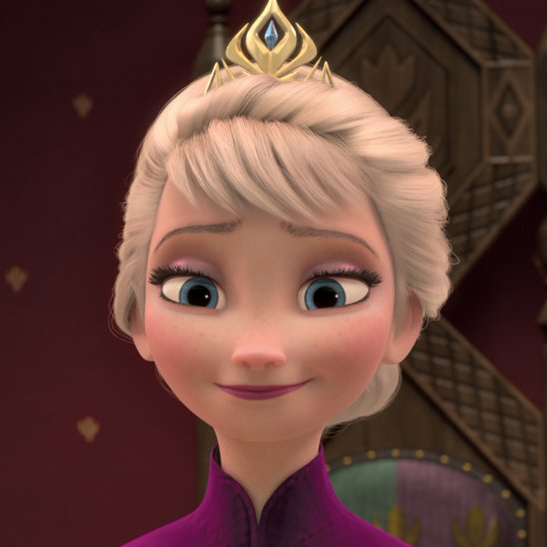
\includegraphics[width=0.3\textwidth]{figs/Introduction/Frozen.png}
\caption{Frozen hair}
\label{fig:frozen}
\end{figure}

In video games \citep{dobrian2006nime}, to solve the problem of realism \citep{broad2021network}, two world leading companies of computer graphics cards - Nvidia \& AMD - have both developed their own hair technologies, HairWorks \& TressFX respectively (see Figure \ref{fig:hair_tech}). They make great efforts to avoid the plastic-molded like hairs appearing in video games. Furthermore, in interactive media and video games, perhaps the most popular facet of any character-customization tool is the ability to customize the appearance of a character in terms of hairstyling, dress and other forms of body modification \citep{Tokui2023surfing}. All of these reasons make hair modelling recognized as a widespread topic in the computer graphics community.

%\pagebreak
